\chapter{Cálculos de Bulk e de Superfície dos Metais\label{apd:metal}}


\section{Paládio (Pd)}
\subsection{Bulk}
%Nos cálculos da estrutura bulk do Paládio foi utilizado uma \textit{base duplo-zeta polarizada} (DZP), no qual o momento angular dos elétrons de valência é descrito por duas funções radiais e uma função de polarização. Dessa forma,  para descrever os elétrons de valência, foi utilizado uma variação otimizadas da base DZP. Nesses cálculos o Método de Minimização utilizado foi o \textit{Gradiente Conjugado (CG)}, o critério de convergência utilizado foi da força $ 0,01$ eV/$\si{\angstrom}$ e o \textit{Mesh Cutoff} utilizado foi 400 Ryd. 

%Nesse sentido, para descrever os elétrons do caroço foi utilizado um pseudopotencial gerado com o funcional PBE com correção relativística e utilizando o Método de Norma Conservada de \textit{Troullier-Martins}. Os raios de corte estão descritos na Tabela \ref{tab:raios_corte} e a configuração de referência utilizada foi:
%As rotinas computacionais da primeira e segunda etapa foram executadas por meio do código \textit{Siesta} \cite{siesta} e a última, por meio do código \textit{Smeagol} \cite{smeagol1} \cite{smeagol2}. As coordenadas dos átomos que compõem as superfícies foram geradas por meio da biblioteca de ferramentas do \textit{Pyhton} denominada \textit{Atomic Simulation Environment} (ASE)\footnote[1]{Documentação do código: \url{https://wiki.fysik.dtu.dk/ase/}.} \cite{ase}. Os funcionais utilizados foram PBE \cite{PBE} e VDW-BH \cite{vdw-bh}

Os cálculos computacionais da estrutura \textit{bulk} do Paládio foram executados por meio do código \textit{Siesta} \cite{siesta}. Os funcionais de troca e correlação utilizados foram GGA-PBE \cite{PBE} e VDW-BH \cite{vdw-bh}. Além disso, utilizamos como método de minimização um algoritmo denominado \textit{Gradiente Conjugado (CG)} e  juntamente com o critério de convergência da força dado por $ 0.001$ eV/$\si{\angstrom}$, os pontos de corte da malha de integração do Siesta foram definidos com o tamanho da malha de 500 Ryd. A integração sobre os pontos do espaço recíproco seguiu o esquema proposto por \citeauthor{pontosk}, com os pontos k dados por $ 20\times20\times20 $ para os cálculos atômicos e de \textit{bulk}.  

Os elétrons de valência foram descritos por duas funções radiais e uma função de polarização, base denominada como \textit{duplo-zeta polarizada} (DZP). Dessa forma,  para descrever os elétrons de valência, utilizamos duas variações otimizadas da base DZP intituladas como DZP$^1$ e  DZP$^2$. Os parâmetros da base DZP$^1$ foram retirados do trabalho de \citeauthor{adrien} e da base DZP$^2$ do artigo de \citeauthor{pseudo_salvador}. 

Nesse sentido, para descrever os elétrons do caroço, utilizamos dois pseudopotenciais distintos obtidos a partir do Método de Norma Conservada de \textit{Troullier-Martins} com correção relativística. Em ambos pseudopotenciais, o cálculo com todos os elétrons foram executados utilizando o funcional PBE e foram denominados como \textit{PS-1} e \textit{PS-S}. O primeiro possui otimizações com correções não lineares no caroço e raios de corte $R_c$ sugeridos por \citeauthor{adrien} e o segundo por \citeauthor{pseudo_salvador}. Em ambos, a configuração de referência utilizada foi a distribuição eletrônica descrita abaixo, de modo que os raios de corte da base e do pseudopotencial, referentes aos respectivos níveis eletrônicos estão indicados na Tabela \ref{tab:raios_corte}.


\begin{equation}
	\bqty{Kr},5s^1,5p^0,4d^9,4f^0
\end{equation}

\begin{table}
	\centering
	\caption{Tabela contendo os valores dos raios de corte (bohr) de acordo com os níveis eletrônicos das bases DZP$ ^1 $ e DZP$ ^2 $ e dos pseudopotenciais PS-S e PS-1. \label{tab:raios_corte}}
	\begin{tabular}{clccccc} 
	\midrule\midrule
		\multicolumn{7}{c}{Raios de Corte -- Paládio}                                                        \\ 
		\midrule
		&  & \multicolumn{2}{c}{Base}            &  & \multicolumn{2}{c}{Pseudopotencial}  \\ 
		\midrule
		Nível Eletrônico &  & DZP$^{1}$ & DZP$^{2}$ &  & PS-S & PS-1                          \\ 
		\midrule
		5s               &  & 8.31/7.13        & 6.60/6.10        &  & 2.48 & 1.79                          \\
		5p               &  & 8.42             & 4.25             &  & 2.48 & 2.48                          \\
		4d               &  & 6.21/ 2.51       & 4.74/ 2.52       &  & 2.16 & 2.48                          \\
		4f               &  & -                & -                &  & 2.48 & 2.48                          \\
		\midrule\midrule
	\end{tabular}
\legend{Fonte: Compilação da autora.}
\end{table}


Os cálculos computacionais realizados pelo código Siesta fornecem informações atômicas e estruturais que podem ser comparadas aos valores obtidos experimentalmente, tais como parâmetro de rede, \emph{bulk modulus} e energia de coesão. O parâmetro de rede determina a distância interatômica na estrutura cristalina e é determinado de acordo com a configuração que fornece a energia mínima da estrutura \emph{bulk}. O \emph{bulk modulus} é uma medida de resistência em relação á compressão de uma substância. A energia de coesão de um cristal é definida como a energia que deve ser adicionada ao cristal a fim de separar sua estrutura em átomos neutros e livres, representada pela expressão \eqref{eq:ebulk}. \cite{kittel}

\begin{equation}\label{eq:ebulk}
	E_{coesão}=E_{sólido}-E_{átomo}
\end{equation}

Dessa forma, utilizando o funcional PBE, foram obtidos os parâmetros estruturais e eletrônicos do Pd \textit{bulk}: \textit{Parâmetro de rede} ($ \si{\angstrom} $), \textit{Bulk Modulus} (GPa) e \textit{Energia de Coesão} (eV), com as bases DZP$ ^1 $ e DZP$^2 $, junto com os pseudpotenciais \textit{PS-1} e \textit{PS-S}. Em posse desses resultados, verificou-se qual combinação de base e pseudopotencial que forneceram os valores mais próximos aos experimentais para o funcional PBE. 

Levando-se em consideração que o problema central desse trabalho é estudar a interface água/metal, é fundamental considerar as forças de dispersão de van der Waals \cite{vdw-func}. Nesse sentido, a fim de descrever e analisar essas interações, obtivemos as propriedades da estrutura bulk do Pd com o funcional de troca e correlação VDW-BH juntamente com a base e o pseudopotencial definidos via cálculos PBE. Isso foi feito pois a convergência do funcional PBE é mais rápida que a do funcional VDW-BH, além do fato de o PBE ser um funcional com resultados bem reportados na literatura \cite{adrien}. 

Os resultados obtidos computacionalmente para os parâmetros de interesse, bem como os valores experimentais estão descritos na Tabela \ref{tab:bulk}. Em relaçao ao \textit{Parâmetro de rede}, a base DZP$^2$ forneceu o valor mais próximo do valor experimental, cerca de $ 1.5\% $ maior, tanto para o pseudopotencial PS-S quanto para o PS-1; enquanto que, a base DZP$^1$ apresentou discrepâncias entre $ 2.3\% $ e $ 2.6\% $. No estudo conduzido por \citeauthor{pseudo_salvador}, onde foi apresentado o pseudopotencial PS-1 e base DZP$^2  $, o valor do parâmetro de rede para o Pd com o funcional PBE foi $ a_{salvador}=3.985\; \AA $, o que condiz com o nosso resultado. Da mesma forma, a base DZP$^2$ forneceu os valores do \textit{Bulk Modulus} mais próximos ao experimental para ambos os pseudopotenciais, com variações entre $6\%$ e $7\%$ menores.

Entretanto, para a \textit{Energia de Coesão} a base DZP$^1$ juntamente com o pseudopotencial PS-1 apresentou o resultado mais próximo ao experimental, com a discrepância de 10 $\%$; ao passo que a maior discrepância foi de $33\%$ dada pela base DZP$^2$+PS-S. \cite{vdw-article}. Dessa forma, escolhemos o a base DZP$^1$ e o pseudopotencial PS-1 para compor os cálculos com o funcional VDW-BH. O critério utilizado nessa escolha foi o valor da Energia de Coesão. Isso ocorreu pois estamos interessados no conjunto que forneça a energia mínima e que seja o mais próximo ao experimental. %Na Figura \ref{fig:fluxo} está representado um fluxograma sintetizando essa etapa do trabalho. 

%Bulk
\begin{table}[H]
	\centering
		\caption{Parâmetros estruturais obtidos com o funcional PBE de acordo com cada base, $DZP^1$ e $DZP^2$, junto a cada pseudopotencial PS-S e PS-1.\label{tab:bulk}}
	\begin{tabular}{ccccc} 
		\hline\hline\addlinespace[3.6pt]
		\multicolumn{5}{c}{\textbf{Valores dos parâmetros obtidos com o funcional PBE}}                                                        \\ \addlinespace[1.5pt]
		\midrule \addlinespace[1.5pt]
		\textit{Pseudo}       & \textit{Base}    & \textit{Par. de rede}$(\si{\angstrom})$ & \textit{Bulk Modulus} (GPa) & \textit{Energia de Coesão} (eV)  \\  
		\midrule
		\multirow{2}{*}{PS-S} &~~~DZP$^1$~~~& 3.98                          & 158 & 4.73          \\ \addlinespace[1pt]
		&~~~DZP$^2$~~~& 3.94                          & 183                      & 5.23                            \\ 
		\midrule
		\multirow{2}{*}{PS-1} &~~~DZP$^1$~~~& 3.97                          & 168                      & 4.34                            \\ 
		\addlinespace[1pt]
		&~~~DZP$^2$~~~& 3.94                          & 181                      & 4.85                            \\ \midrule	\multicolumn{5}{c}{\textbf{Valores dos parâmetros obtidos com o funcional VDW-BH}}    \\ \addlinespace[1pt]
		\midrule \addlinespace[3pt]
		PS-1 & DZP$ ^1 $&3.91 &199& 4.93                                                     \\ 
		\midrule
		\multicolumn{2}{c}{\textbf{Exp.}\tablefootnote[2]{CRC Handbook of Chemistry and Physics version 2008.}}        & \textbf{3.88}                          & \textbf{195}                     & \textbf{3.94}                             \\
		\hline\hline
	\end{tabular}
\legend{Fonte: Compilação da autora}
\end{table}



%\begin{figure}[H]
%	\centering
%	\includegraphics[scale=0.6]{figs/funcional.pdf}
%	\caption{\textit{Fluxograma ilustrando a escolha do pseudopotencial PS-1 e da base DZP$ ^1 $. Após obter os resultados com o funcional PBE e as diversas combinações, representado à esquerda, comparou-se com o valor experimental, escolhendo a combinação adequada para os cálculos VDW-BH (lado direito). Fonte: Compilação da autora.} }
%	\label{fig:fluxo}
%\end{figure}

Em relação aos valores obtidos com o funcional VDW-BH, é possível observar uma melhoria nos resultados obtidos para o pseudopotencial PS-1 e a base DZP$ ^1 $. Por exemplo, a discrepância do parâmetro de rede em relação ao valor experimental foi $ \delta_{PS-1}=0.03 \si{\angstrom}$, caracterizando uma redução de 0.06 em comparação ao funcional PBE. Além disso, no trabalho reportado por \citeauthor{vdw-bh}, o parâmetro de rede obtido com esse funcional para o Pd foi $ a_{vdw-BH}=3.89\si{\angstrom} $, próximo ao valor que obtivemos. Para o parâmetro bulk modulus, o valor obtido foi superior em 4 GPa em comparação ao valor experimental, o que indica uma melhor concordância do que o valor obtido por \citeauthor{vdw-bh} $ B_{vdw-bh}=207 $ GPa.  Por outro lado, para a energia de coesão a diferença foi 0.99 eV em relação ao valor experimental. Todavia, esse valor é da mesma ordem de grandeza do valor obtido no trabalho realizado por \citeauthor{vdw-article} com outro funcional da família vdW, dado por 4.37 eV.

Assim, de acordo com o critério de energia e após comparar bases e pseudopotenciais para a descrição da estrutura \textit{bulk} do Pd com o funcional PBE, obtemos que a base DZP$^1$ e o pseudopotencial PS-1 forneceram o menor valor da energia. Com esse conjunto, realizamos os cálculos com o funcional VDW-BH, cujo valor da energia de coesão foi maior que com PBE.


\subsection{Superfície}
A construção do modelo ideal de uma superfície pode ser pensado a partir de um cristal infinito em duas dimensões e finito ao longo da direção normal, no qual o arranjo atômico da estrutura cristalina \textit{bulk} é preservado; esse modelo é denominado \textit{bulk-terminated}. Para implementar esses modelos nos cálculos computacionais aplica-se as condições periódicas de contorno nas duas dimensões e, na direção normal, repete-se as camadas após uma camada de vácuo. Tal configuração é denominada por  \textit{slab}. 

Os cálculos de superfície do Pd foram realizados no código Siesta com os funcionais PBE e VDW-BH. O método de Minimização utilizado foi o CG com o critério da força dado por $ 0.001\;\text{eV}/\AA$ e o \textit{Mesh Cutoff} de 400 Ryd. Assim como no cálculo de \textit{bulk}, utilizou-se as bases DZP$ ^1 $ e DZP$^2  $ juntamente com os pseudopotenciais PS-S e PS-1 para os cálculos utilizando o funcional PBE. Em seguida, a partir dos resultados das combinações de bases e pseudopotenciais obtidos com o PBE, realizou-se os cálculos com o funcional VDW-BH.

Para descrever as superfícies de Pd, utilizamos duas estruturas \textit{slab}, cuja ordenação atômica da célula unitária era composta por $ 4\times 4\times 4$ e $ 6\times 6\times 4 $ átomos nas coordenadas \textit{x}, \textit{y} e \textit{z}, respectivamente,  e vácuo de $ 20\; \si{\angstrom}$. A orientação dos planos cristalográficos escolhida para as superfícies foi a orientação (111), uma vez que corresponde a orientação com a maior densidade de átomos. %As coordenadas atômicos foram geradas por meio da biblioteca de ferramentas do \textit{Pyhton} denominada \textit{Atomic Simulation Environment} (ASE)\footnote[1]{Documentação do código: \url{https://wiki.fysik.dtu.dk/ase/}.} \cite{ase}.  

Vale ressaltar que utilizamos diferentes tamanhos de células unitárias, pois os cálculos de energia total de sistemas periódicos utilizando condições periódicas de contorno são influenciados pelo tamanho da célula unitária. Em particular, para sistemas envolvendo a interface água/metal- tais como os que serão abordados na próxima sessão- a periodicidade imposta pode causar uma interação indesejada entre moléculas polares em células adjacentes, o que afeta tanto as energias, quanto as geometrias dos sistemas \cite{adrien}. Nesse sentido, considerando a adsorção de estruturas de água adsorvidas no Pd, nessa etapa foram analisados as propriedades de um slab de metal com dois tamanhos diferentes de células unitárias.

A grandeza física mensurada e analisada nessa etapa foi o valor da \textit{Função Trabalho} (W), de modo que, esse valor foi calculado para cada conjunto e para cada tamanho de superfície. A definição da Função Trabalho é a energia mínima necessária para remover um elétron do interior de um cristal para um ponto no vácuo sujeito ao campo eletrostático gerado pela superfície e é expressa por:
\begin{equation}\label{eq:work}
	W=-E_F+W_s
\end{equation}
onde $E_f$ é a \textit{Energia de Fermi} previamente calculada para um cristal infinito e $W_s$ é a energia de um elétron em repouso no vácuo e próximo à superfície.

Computacionalmente esse parâmetro é calculado a partir do arquivo de saída gerado pelo Siesta que contém as informações da energia potencial do cristal em cada ponto ao longo da direção normal \textit{z}. Assim, por meio do utilitário fornecido pelo Siesta, são obtidos os arquivos contendo a média planar e a média macroscópica da energia potencial, respectivamente de acordo com a expressões:
\begin{equation}\label{eq:planar}
	\bar{V}(z)=\frac{1}{S}\int_{S}\dd{x}\dd{y}V(\vb{r})
\end{equation}

\begin{equation}\label{eq:macro}
	\bar{\bar{V}}(z)\int \dd{z'}f(z-z')\bar{V}(z')
\end{equation}
onde $ f(z-z') $ é uma função de amortecimento suave dada por \footnote{Para mais detalhes, consultar \citeauthor{planar}.}  e:
\begin{equation}
	f(z-z')=\int \dd{z''}\omega_{l_1}(z-z'')\omega_{l_2}(z''-z')
\end{equation}

Na Figura \ref{fig:work1} está representado o potencial de uma superfície de tamanho  $4\times4\times4$ e o significado de \textit{W}. Além disso, é possível observar as alterações na Energia Potencial nos pontos correspondentes às posições dos átomos da superfície, bem como as distorções devido à quebra de simetria de um cristal \textit{bulk} para uma superfície presentes na camada próxima ao vácuo. Assim, utilizando a Equação \eqref{eq:work} e as curvas de potencial, foram obtidos os resultados de W para os diferentes funcionais, apresentados na Tabela \ref{tab:work}. 

Considerando as bases DZP$^1  $ e DZP$ ^2 $, tem-se que os valores mais próximos à função trabalho experimental do Pd (111) foram obtidos para a base DZP$^1$, com ênfase para o pseudopotencial PS-1, cujas discrepâncias foram $\delta_{4\times4\times4}=0.30$ eV e $\delta_{6\times6\times4}=0.32$ eV. Por outro lado, a base DZP$^2$ forneceu resultados divergentes do experimental, com discrepâncias variando entre 1.4 a 1.8 eV. Os valores obtidos com a base DZP$ ^1 $ e o pseudopotencial PS-1 para o funcional PBE estão de acordo com o valor obtido por \citeauthor{work} para o Pd - fcc(111)- com esse funcional, $ W_{ref}=5.32 $ eV.
\begin{table}[h!]
	\centering
		\caption{Tabela contendo os valores obtidos para a Função Trabalho em elétron-Volt (eV).\label{tab:work}}
	\begin{tabular}{cccc} 
		\hline\hline\addlinespace[3.6pt]
		\multicolumn{4}{c}{\textbf{Funcional PBE}}                                                                                         \\ \addlinespace[2pt]
		\midrule \addlinespace[2pt]
		\textit{Pseudopotencial} & Base                                                               & Superfície        & Função Trabalho (eV)  \\ 
		\midrule
		\multirow{4}{*}{PS-S}    & \multirow{2}{*}{DZP$^1$}                                           & $4\times4\times4$ & 5.15                 \\ 
		\cdashline{3-4}[1pt/1pt] \addlinespace[3pt]
		&                                                                    & $6\times6\times4$ & 5.13                 \\ 
		\cmidrule{2-4}
		& \multirow{2}{*}{DZP$^2$}                                           & $4\times4\times4$ & 3.87                 \\ 
		\cdashline{3-4}[1pt/1pt]\addlinespace[3pt]
		&                                                                    & $6\times6\times4$ & 3.80                 \\ 
		\midrule
		\multirow{4}{*}{PS-1}    & \multirow{2}{*}{\begin{tabular}[c]{@{}c@{}}DZP$^1$\\\end{tabular}} & $4\times4\times4$ & 5.30                 \\ 
		\cdashline{3-4}[1pt/1pt]\addlinespace[3pt]
		&                                                                    & $6\times6\times4$ & 5.28                 \\ 
		\cmidrule{2-4}
		& \multirow{2}{*}{DZP$^2$}                                           & $4\times4\times4$ & 4.19             \\ 
		\cdashline{3-4}[1pt/1pt]\addlinespace[3pt]
		&                                                                    & $6\times6\times4$ & 4.15                 \\ 	\hline\addlinespace[3pt]
		\multicolumn{4}{c}{\textbf{Funcional VDW-BH}}                                                                                         \\
		\midrule
		\multirow{2}{*}{PS-1}    & \multirow{2}{*}{\begin{tabular}[c]{@{}c@{}}DZP$^1$\\\end{tabular}} & $4\times4\times4$ & 5.43                 \\ 
		\cdashline{3-4}[1pt/1pt]\addlinespace[3pt]
		&                                                                    & $6\times6\times4$ &     5.46           \\ 
		\midrule
		\multicolumn{3}{c}{\textbf{Exp.}\tablefootnote[2]{CRC Handbook of Chemistry and Physics version 2008, p. 12–114.}}                                                                                          & \textbf{5.60}                 \\
		\hline\hline
	\end{tabular}
	\legend{Fonte: Compilação da autora}
\end{table}
\begin{figure}[h!]
	\centering
	\caption{Curva de energia potencial pela distância no eixo z de uma superfície de Pd de tamanho $4\times4\times4$. No gráfico $ E_f $ corresponde à Energia de Fermi do sistema e W é a função trabalho; as linhas tracejadas representam a caixa unitária.}
	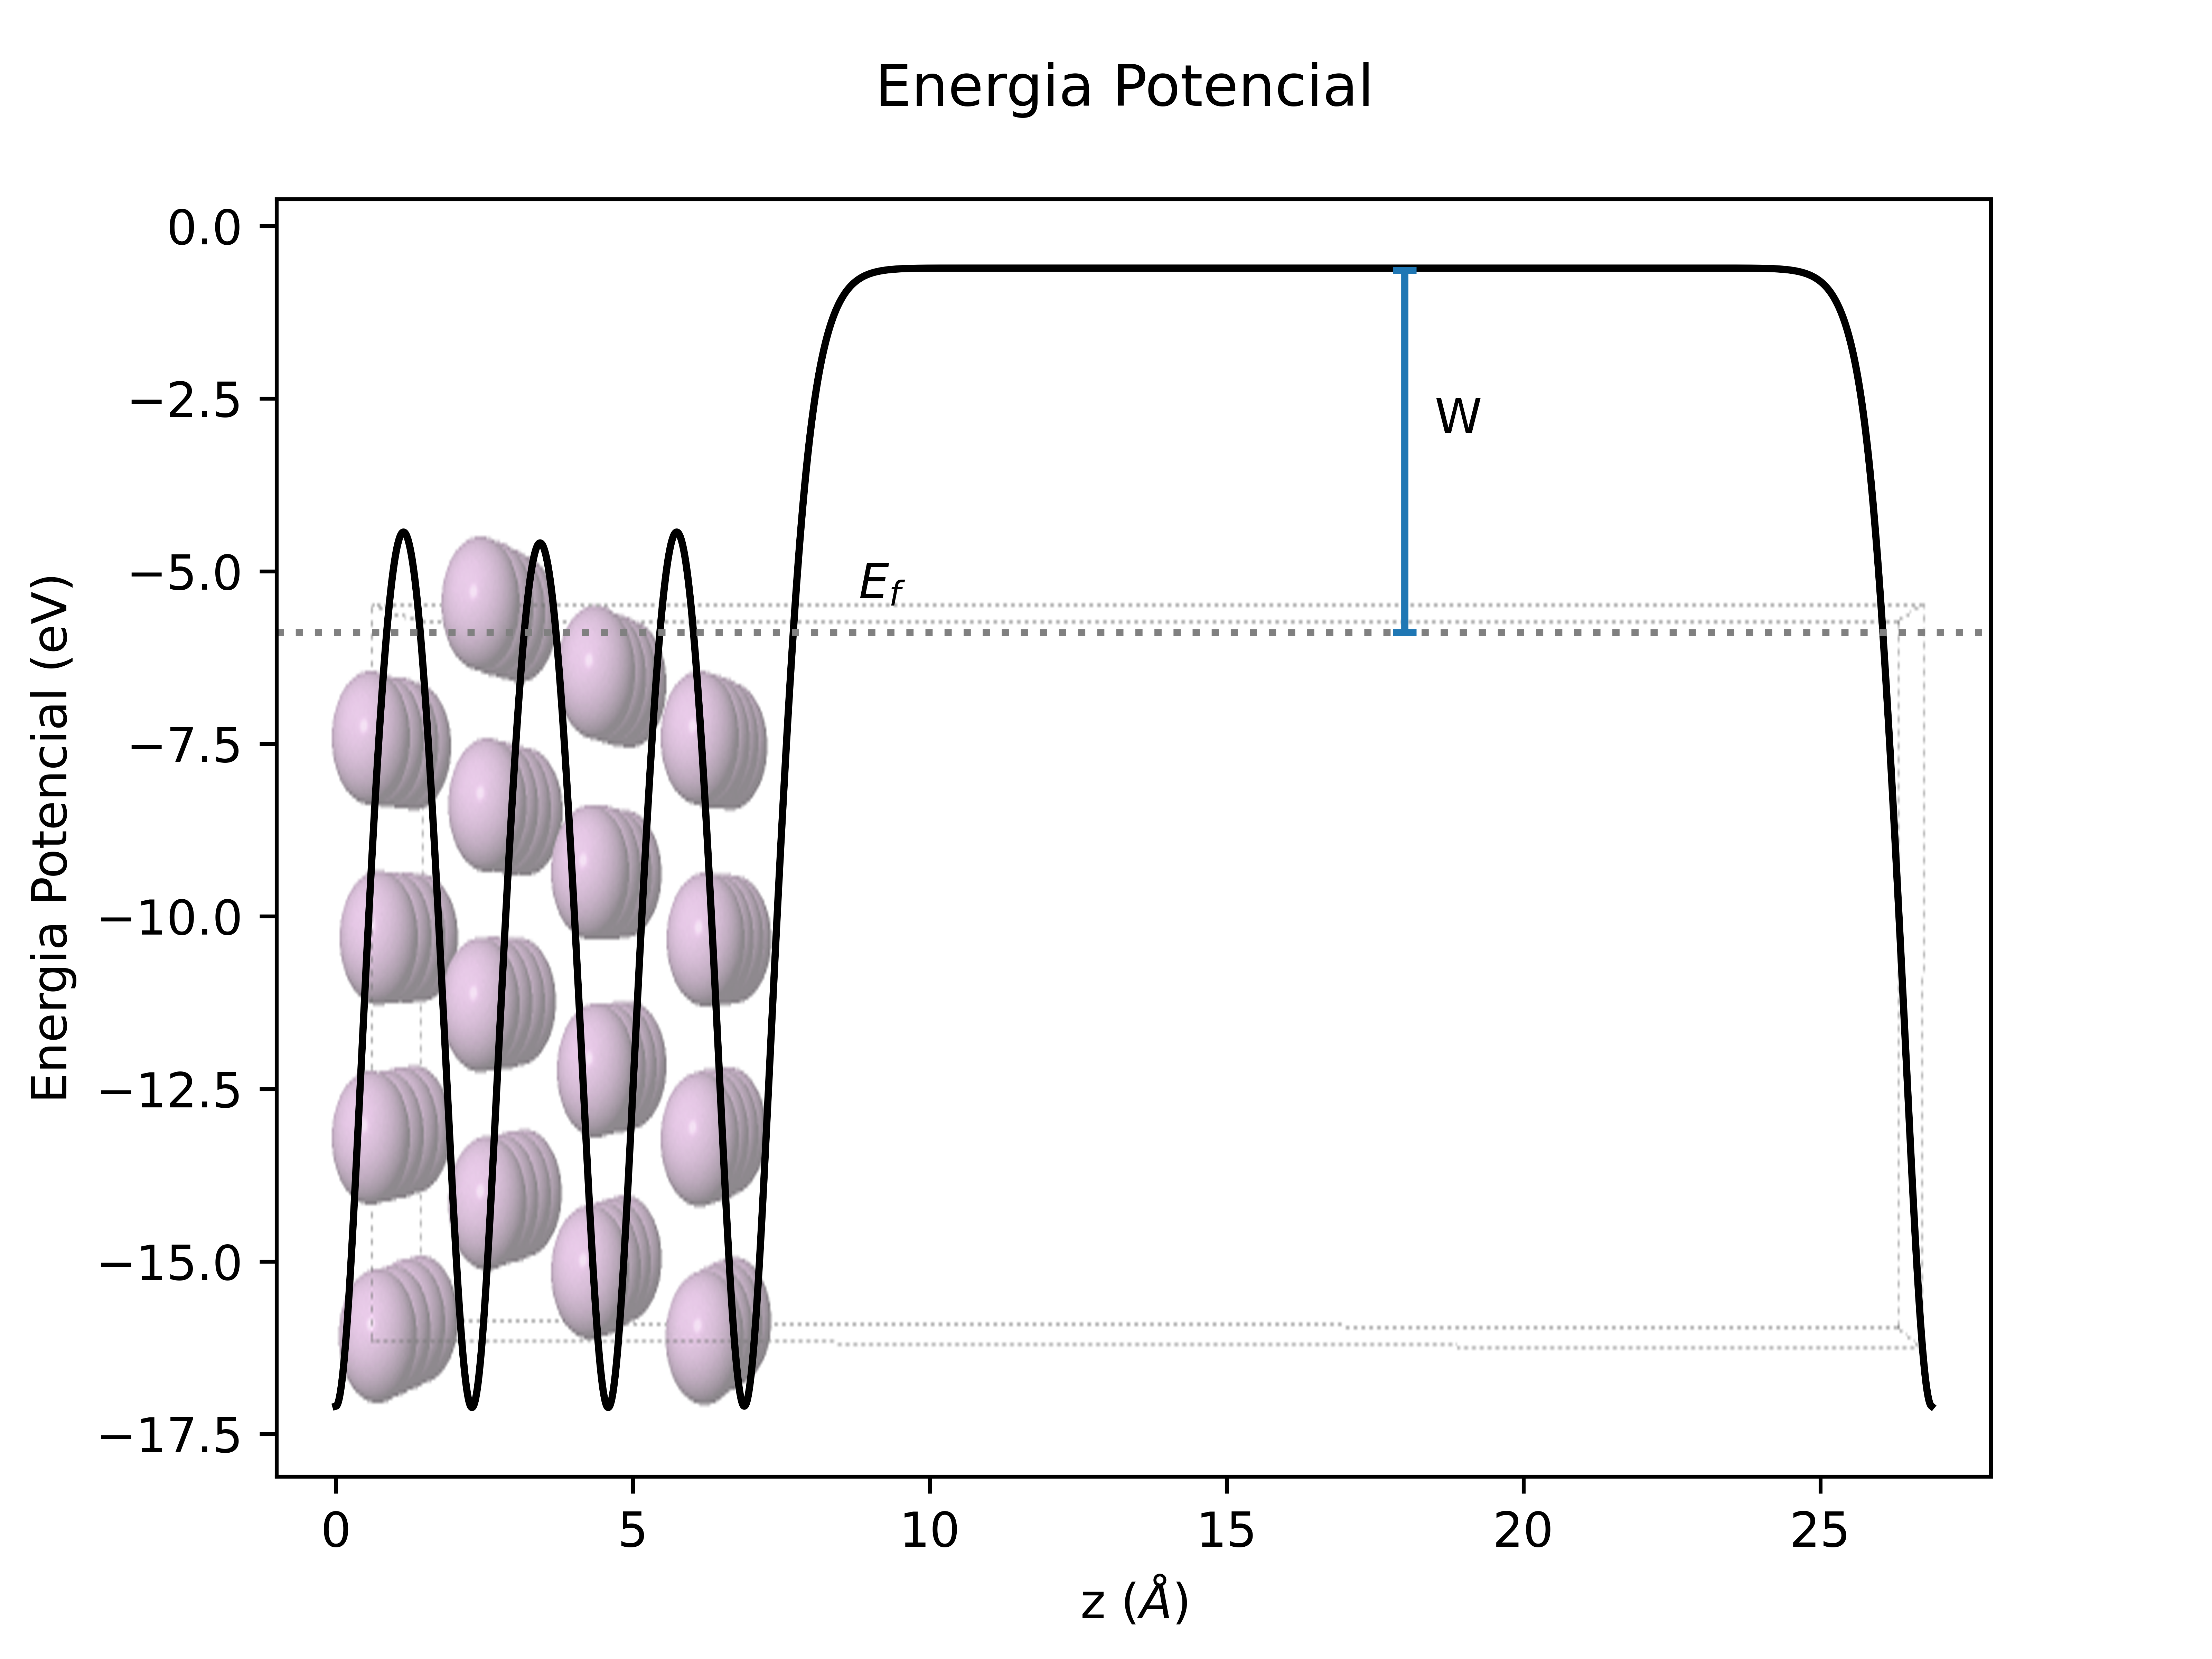
\includegraphics[scale=0.8]{figs/work2.png}
	\legend{Fonte: compilação da autora.}
	\label{fig:work1}
\end{figure}

Assim como para o cálculo de bulk, os valores obtidos com o pseudopotencial PS-1 e base DZP$ ^1 $ com o funcional PBE foram os mais próximos ao experimental, de modo que os cálculos envolvendo o funcional VDW-BH foram realizados com esse conjunto de descritores. Comparando com os valores obtidos via PBE, observa-se uma melhoria nos valores fornecidos pelo funcional VDW-BH com os resultados mais próximos ao experimental cujas discrepâncias foram $\delta_{4\times4\times4}=0.17$ eV e $\delta_{6\times6\times4}=0.14$ eV.



Portanto, a partir da caracterização do Pd é possível concluir que o funcional VDW-BH fornece resultados melhores que o funcional PBE em alguns resultados analisados. Isso constitui uma vantagem, visto que é esperado que esse funcional seja mais sensível às interações água-Pd, corroborando assim para a descrição posterior da água adsorvida no metal. Além disso, a partir dos resultados obtidos nessa etapa, definiu-se o conjunto de base e pseudopotencial que melhor descrevem as propriedades eletrônicas e estruturais do paládio, tanto para a estrutura \textit{bulk}, quanto para a estrutura \textit{slab}. 


\section{Raios de Corte}
Para descrever as moléculas de água durante as simulações foi utilizado bases DZP e pseudpotenciais de norma conservada de acordo com a norma de \textit{Troulier-Martins}. Assim, os raios de corte do oxigênio e do hidrogênio estão descritos nas Tabelas \ref{tab:o} e \ref{tab:h}, respectivamente. Além disso, foi investigado o efeito do potencial sobre eletrodos metálicos de ouro, cujos raios de corte estão descritos na Tabela \ref{tab:au}. Nas simulações com a superfície metálicas de Au, foi utilizado a base DZP$ ^{Au} $ para descrever os eletrodos e a base DZP$^{Aus}  $ para descrever a região de espalhamento.

\begin{table}[H]
	\centering
		\caption{Raios de Corte (bohr) da base DZP e do pseudopotencial utilizados para descrever os átomos de oxigênio.\label{tab:o}}
	\begin{tabular}{clccc} 
		\hline\hline
		\multicolumn{5}{c}{Raios de Corte - Oxigênio (O)}          \\ 
		\midrule
		Nível Eletrônico &  & DZP &  & Pseudopotencial  \\ 
		\midrule
		2s               &  & 4.51/2.64  &  & 1.14             \\
		2p               &  & 6.15/2.59  &  & 1.14             \\
		3d               &  & 3.54       &  & 1.14             \\
		4f               &  & -          &  & 1.14             \\
		\hline\hline
	\end{tabular}
\end{table}

\begin{table}[H]
	\centering
			\caption{Raios de Corte (bohr) da base DZP e do pseudopotencial utilizados para descrever os átomos de hidrogênio.\label{tab:h}}
	\begin{tabular}{clccc} 
		\hline\hline
		\multicolumn{5}{c}{Raios de Corte - Hidrogênio (H)}    \\ 
		\midrule
		Nível Eletrônico &  & DZP &  & Pseudopotencial  \\ 
		\midrule
		1s               &  & 4.20/1.84  &  & 1.25             \\
		2p               &  & 3.52       &  & 1.25             \\
		3d               &  & -          &  & 1.25             \\
		4f               &  & -          &  & 1.25             \\
		\hline\hline
	\end{tabular}
\end{table}

\begin{table}[H]
	\centering
	\caption{Raios de Corte (bohr) da base DZP e do pseudopotencial utilizados para descrever os átomos de ouro.\label{tab:au}}
	\begin{tabular}{clcccc} 
		\hline\hline
		\multicolumn{6}{c}{Raios de Corte - Ouro (Au)}                                                \\ 
		\midrule
		\multicolumn{1}{l}{Nível Eletrônico} &  & DZP$^{Au}$ & DZP$^{Aus}$ &  &      Pseudopotencial             \\ 
		\midrule
		6s                                   &  & 7.25/5.79  & 9.08/5.79   &  & 2.32             \\
		6p                                   &  & -          & -           &  & 2.29             \\
		5d                                   &  & 5.11/2.87  & 6.56/2.87   &  & 2.24             \\
		5f                                   &  & -          & -           &  & 2.00             \\
		\hline\hline
	\end{tabular}
\end{table}
